% =============================================================================
% fig_dag_mediacao.tex — DAG de Mediação da Exposição à IA sobre a Informalidade
%
% Mostra: a exposição ocupacional à IA (X) reduz a informalidade (Y) através
% de dois canais fundamentais:
% 1. Canal indireto via escolaridade (M) — composição de capital humano (37,2%)
% 2. Canal direto via capital organizacional corporativo das firmas formais (62,8%)
%
% Compilar standalone via: xelatex fig_dag_mediacao.tex (ou pdflatex)
% =============================================================================

\documentclass[border=6pt]{standalone}
\usepackage[utf8]{inputenc}
\usepackage[T1]{fontenc}
\usepackage{amsmath,amssymb}
\usepackage{tikz}
\usetikzlibrary{arrows.meta, positioning, calc}

\definecolor{node-fill}{HTML}{F8FAFC}
\definecolor{node-border}{HTML}{002855}
\definecolor{arrow-slate}{HTML}{334155}
\definecolor{direct-red}{HTML}{B91C1C}
\definecolor{gold-accent}{HTML}{B9975B}

\tikzset{
  dag-node/.style={
    draw=node-border, fill=node-fill, rounded corners=3pt, line width=1.1pt,
    minimum width=2.9cm, minimum height=1.2cm, text width=2.7cm,
    align=center, font=\small\linespread{1.0}\selectfont
  },
  dag-edge/.style={-{Latex[length=3.0mm, width=2.0mm]}, line width=1.3pt, draw=arrow-slate},
  direct-edge/.style={-{Latex[length=3.0mm, width=2.0mm]}, line width=1.5pt, draw=direct-red}
}

% -----------------------------------------------------------------------------
% Diagrama: X -> M -> Y caminho de mediação; efeito direto X -> Y curvado abaixo.
% Coordenadas:
%   X at (0, 0)     -- Exposição ocupacional à IA (theta_j)
%   M at (4.2, 2.4) -- Escolaridade / Capital Humano (e_i)
%   Y at (8.4, 0)   -- Informalidade ocupacional (informal_i)
% Corda X-Y = 8.4cm. Curvatura de 28° para baixo evita qualquer sobreposição.
% -----------------------------------------------------------------------------

\begin{document}
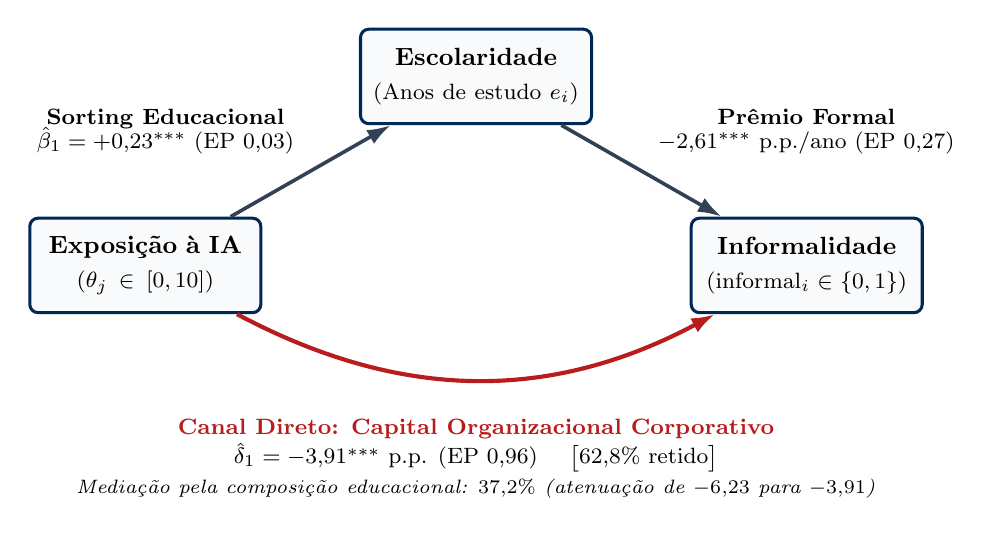
\begin{tikzpicture}
  % Nós estruturais (Regra P1: dimensões explícitas)
  \node[dag-node] (X) at (0, 0) {
    \textbf{Exposição à IA}\\[0.15em]
    \footnotesize $(\theta_j \in [0, 10])$
  };

  \node[dag-node] (M) at (4.2, 2.4) {
    \textbf{Escolaridade}\\[0.15em]
    \footnotesize (Anos de estudo $e_i$)
  };

  \node[dag-node] (Y) at (8.4, 0) {
    \textbf{Informalidade}\\[0.15em]
    \footnotesize $(\text{informal}_i \in \{0, 1\})$
  };

  % Arestas de mediação indireta (Regra P4: palavras direcionais)
  \draw[dag-edge] (X) -- (M)
    node[midway, above left=0.1cm, align=center, font=\footnotesize] {
      \textbf{Sorting Educacional}\\[-0.1em]
      $\hat{\beta}_1 = +0{,}23^{***}$ (EP 0{,}03)
    };

  \draw[dag-edge] (M) -- (Y)
    node[midway, above right=0.1cm, align=center, font=\footnotesize] {
      \textbf{Prêmio Formal}\\[-0.1em]
      $-2{,}61^{***}$ p.p./ano (EP 0{,}27)
    };

  % Efeito direto não mediado curvado abaixo (Regra P4: palavras direcionais)
  \draw[direct-edge] (X) to[bend right=28]
    node[midway, below=0.35cm, align=center, font=\footnotesize] {
      \textcolor{direct-red}{\textbf{Canal Direto: Capital Organizacional Corporativo}}\\[0.15em]
      $\hat{\delta}_1 = -3{,}91^{***}$ p.p. (EP 0{,}96) \quad $\big[62{,}8\%$ retido$\big]$\\[0.15em]
      \scriptsize \textit{Mediação pela composição educacional: $37{,}2\%$ (atenuação de $-6{,}23$ para $-3{,}91$)}
    } (Y);
\end{tikzpicture}
\end{document}
